\section{Results and Analysis}

Table~\ref{tab:fid-scores} summarizes the mean and standard deviation of the FID scores obtained for each model across five independent runs.

\begin{table}[h]
\centering
\caption{Fréchet Inception Distance (FID) results over 5 runs. Lower is better.}\label{tab:fid-scores}
\begin{tabular}{lcc}
\toprule
\textbf{Model} & \textbf{Mean} & \textbf{Std. Dev.} \\
\midrule
VAE        & 201.73 & 0.23 \\
GAN        & 180.57 & 0.71 \\
Diffusion  & 423.70 & 0.64 \\
\bottomrule
\end{tabular}
\end{table}

\begin{figure}
    \centering

    \begin{minipage}[t]{0.48\textwidth}
        \centering
        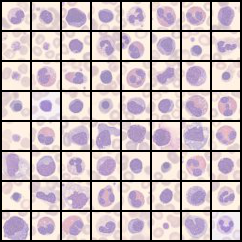
\includegraphics[width=\linewidth]{images/real.png}
        (a) Real Images
    \end{minipage}
    \hfill
    \begin{minipage}[t]{0.48\textwidth}
        \centering
        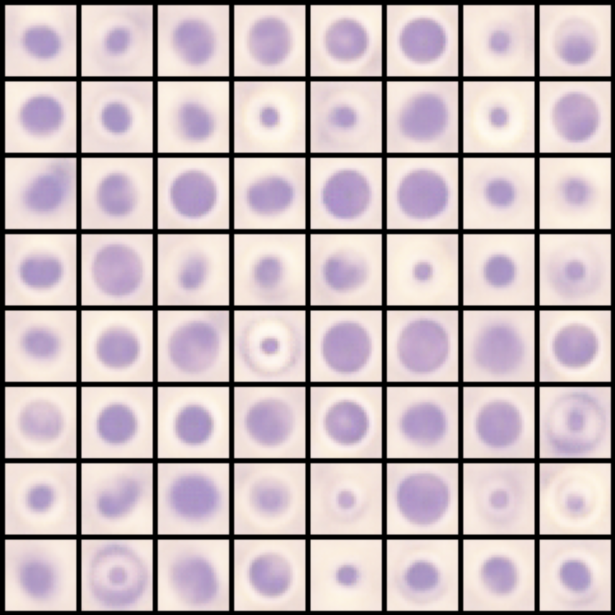
\includegraphics[width=\linewidth]{images/vae.png}
        (b) VAE Samples
    \end{minipage}

    \vspace{0.5em}

    \begin{minipage}[t]{0.48\textwidth}
        \centering
        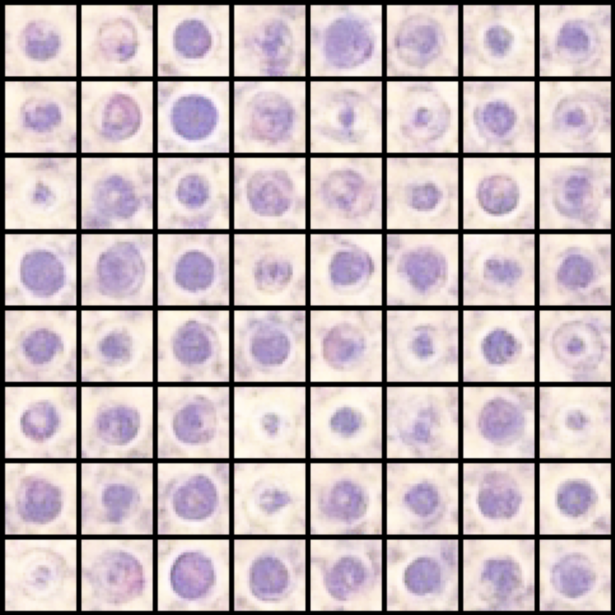
\includegraphics[width=\linewidth]{images/gan.png}
        (c) GAN Samples
    \end{minipage}
    \hfill
    \begin{minipage}[t]{0.48\textwidth}
        \centering
        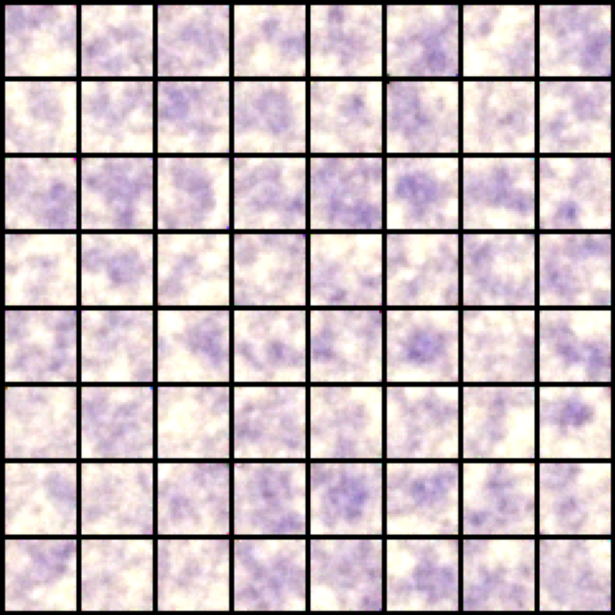
\includegraphics[width=\linewidth]{images/diffusion.png}
        (d) Diffusion Samples
    \end{minipage}

    \caption{Qualitative comparison of real and generated blood cell images.}\label{fig:model-comparison}
\end{figure}

Figure~\ref{fig:model-comparison} shows both the real images and the visual samples generated by each model. The results reveal clear qualitative differences. The VAE samples exhibit smooth but often blurry outputs due to its probabilistic reconstruction objective. Diffusion models produce a lump of blobs, barely resembling a blood cell. GANs generate highly detailed and diverse samples, closely resembling real blood cells.

Overall, GANs achieve the best quantitative and qualitative performance, indicating superior capability in modeling complex visual structures present in biomedical data.
